\section{Experimental Results}
\label{s:experiments}
The following Section presents a representative sample of our experiments. The work \cite{Pro:26} contains a range of additional results.

\subsection{Data} \label{s:data}
In the experiment, we have selected 100 stocks with the highest average return in the year 2021, among the Fortune500 (S\&P500) companies. Of those 100, we have further filtered out the 20 least pair-wise correlated among them. The experiment was conducted on more than 100 portfolios containing 8 to 12 randomly selected stocks out of these twenty. \bl{Fig. \ref{fig:corr_matrix} presents the correlation matrix for these selected stocks}. This was done mainly to reduce bias and have a methodological way to select the stocks for our portfolios.
The optimisation ran on market data from October 2022 to October 2025, which is about 750 trading days.  The first 125 days were used to collect $\bar{\mat{V}}_{\bar{t}}$ used to obtain the optimal prior $\mat{V}_0$, $\ref{s:prior}$. The following 125 trading days were to collect more data to run the structure estimation, $\ref{s:SE}$. The remaining 500 days were to run the optimisation itself.

\subsection{Optional Parameters} \label{s:options}
The optional parameters primarily concern structure estimation and forgetting.

The parameters for our implementation of the genetic algorithm are taken as batch size $=8$, $p_{mut} = 0.5$, and the decay rate for $p_{mut}$ was set at $\alpha_{decay}=0.992$. The genetic algorithm ran for 500 iterations with each new portfolio.

The regressors in $\bar{z}_{t}=\bar{x}_{t-1}$, among which the structure estimation selects significant ones, are the returns in the last 10 trading days, the difference between long- and short-term exponential moving averages, sine functions with periods of 10, 30 and 90 days, and an intercept.

We performed a $2^k$ experiment design \cite{4736103} to determine a good choice of remaining parameters, which are left to the user's responsibility. The data we used for this task were from 2021 to 2022. The model parameters from Secs.\ $\ref{s:prior}$, $\ref{s:forgetting}$ were set to $\alpha_0 = 0.09$, $\beta_0 = 0.5$, $\mu = 0.9$.

\subsection{Metrics and Base-Line Policies} \label{s:metrics}
The relevant metrics for portfolio optimisation reflect the primary goal of maximising returns and the secondary goal of achieving low variance in those returns. The chosen metrics are: $\bullet$ maximum draw-down (the largest percentage loss experienced); $\bullet$ total return (or cumulative wealth);
$\bullet$ average returns (annualized);  $\bullet$ an average return variance (Var(returns)); and $\bullet$ Sharp ratio (SR$=
\mbox{average return}\,/\sqrt{\mbox{average return variance}}$).

Figures exploit the mean and median of these metrics evaluated across all runs, cf.\ Sec.\
\ref{s:data}. Tables show the mean and median values of the metrics considered.

Our algorithm is called Risk Averse (RA) and starts with uniform allocation. It considers $0.2\%$ cost for each transaction, which is low but common. Note that the majority of brokers offer fractional shares, so we don't have to care about that either.

\bl{Two types of portfolio choice serve us for comparison. The first, called Ideal Uniform (IU) and it always maintains $1/N$ allocation in each stock and does not pay transaction costs at all, hence the name Ideal. The second, called Uniform (U), uniformly allocates funds to all assets as well but pays transaction costs. Transaction costs for this portfolio are taken as 5bps (5 basis points) for each reallocation.}

\subsection{Results and Discussion} \label{s:results}
The qualitative comparison provides figures. Plots \ref{fig:pareto_plot_u} of average returns vs.\ average deviation of returns, with indicated maximum draw-down, compare our algorithm with the Ideal Uniform baseline. Each \bl{spot} reflects one portfolio.

The median of the time evolutions of $\ln(\mbox{SR})$ in Fig.\
 \ref{fig:sr_plot_ideal}, \ref{fig:sr_plot_u} complements the qualitative picture.

 Tables \ref{tab:metrics_mean} and \ref{tab:metrics_median} numerically show that our policy, despite paying transaction costs, \bl{exhibits behavior closer to the Ideal Uniform} policy that does not pay these costs. We are truly risk-averse as we improve maximum draw-down and consequently also total return. Compared to the Uniform policy, that pays transaction costs, our improvements are even more visible.

\begin{figure}[ht!]
    \begin{minipage}{0.45\textwidth}
    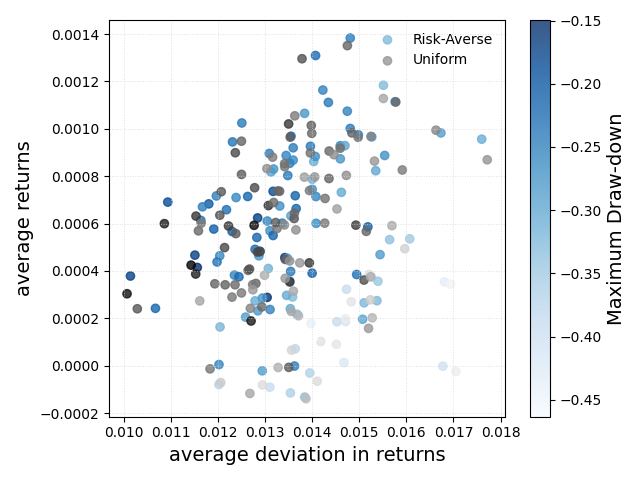
\includegraphics[width=\linewidth]{Images/ar_vs_ad_plot_HER_09mu.png}
    \caption{Average return vs. average deviation of returns for Risk Averse and theoretically ideal Uniform portfolios.}
    \label{fig:pareto_plot}
    \end{minipage}
    \vfill

    \begin{minipage}{0.45\textwidth}
    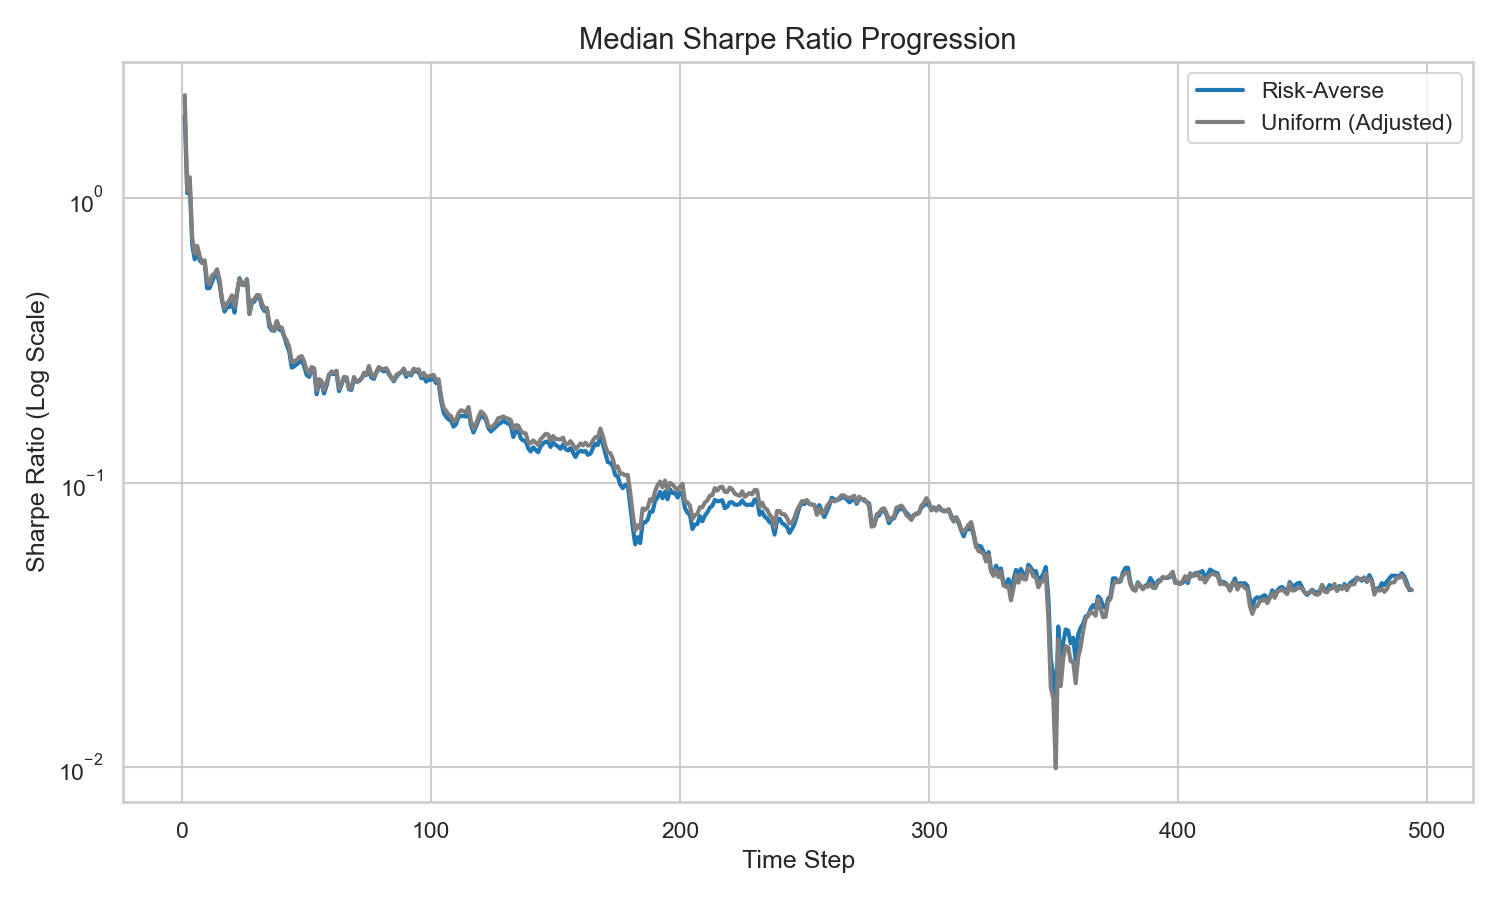
\includegraphics[width=\linewidth]{Images/median_sr_no_trc_u.png}
    \caption{Median Sharpe ratio progression for Risk Averse \& theoretically ideal Uniform portfolios.}
    \label{fig:sr_plot_ideal}
    \end{minipage}
    \vfill

    \begin{minipage}{0.45\textwidth}
    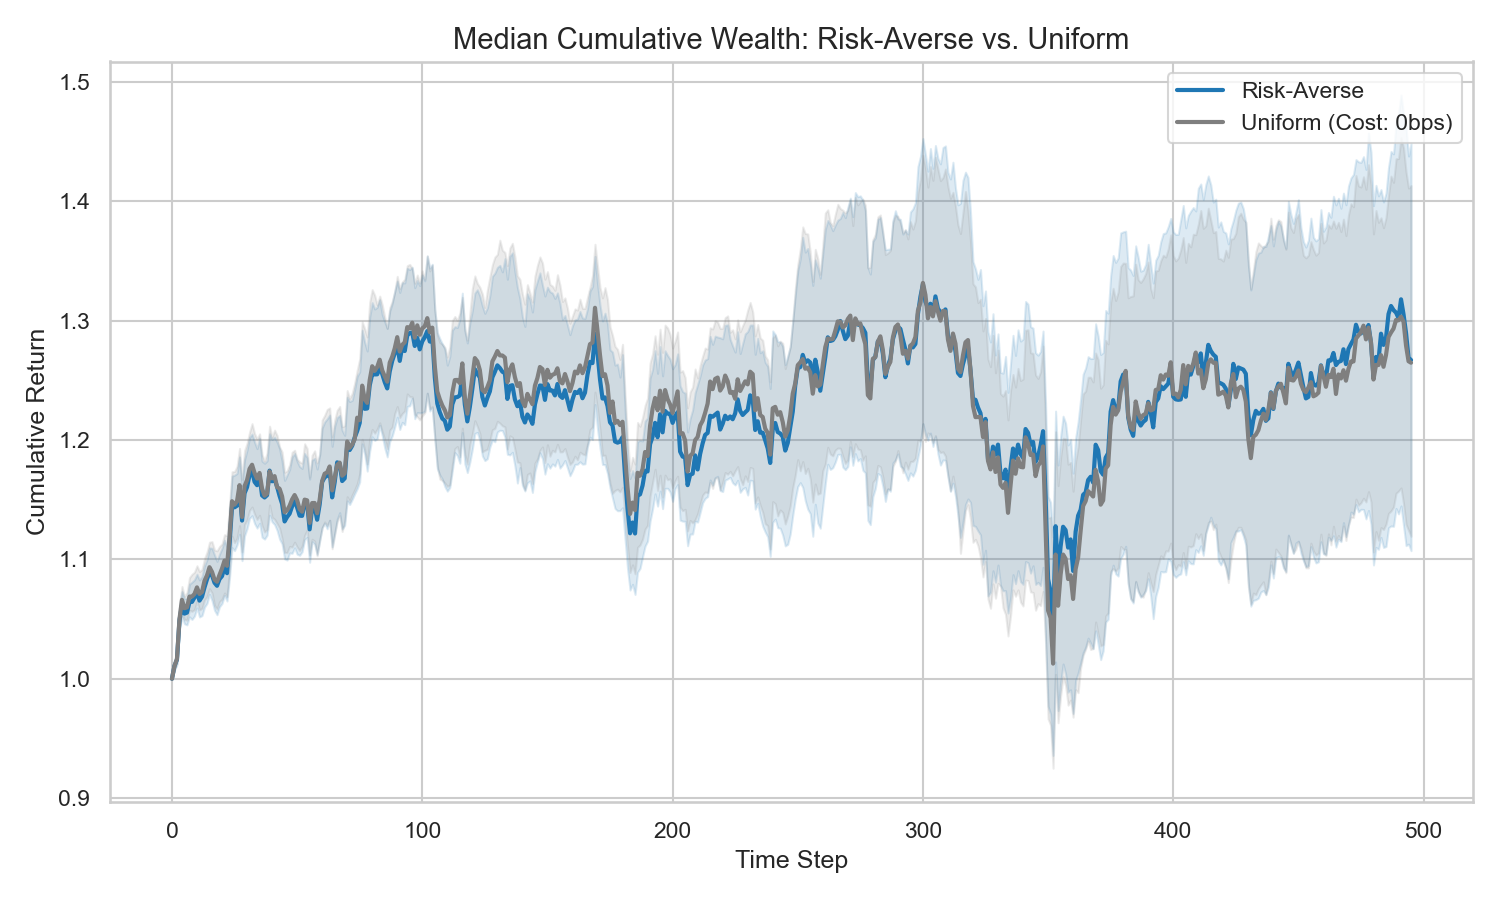
\includegraphics[width=\linewidth]{Images/cum_wealth_no_trc_u.png}
    \caption{Cumulative wealth for Risk Averse \& theoretically ideal Uniform portfolios.}
    \label{fig:cum_wealth_ideal}
    \end{minipage}
\end{figure}

\begin{table}[ht!]
   \begin{minipage}{0.48\textwidth}
  % \centering
        \begin{tabular}{||l|r r r||} % Example table
        \hline
        & RA & IU & U\\
        \hline
        max draw-down & -\textbf{0.273} & -0.281 & -0.339\\
        total return & \textbf{1.278} & 1.262 & 0.985\\
        average return & 5.62e-4 & 5.37e-4 & 0.37e-4\\
        average return var. & 1.88e-4 & 1.86e-4 & 1.86e-4\\
        SR & 0.041 & 0.039 & 0.005\\
        \hline
     \end{tabular}
  \end{minipage}
  \caption{Comparison of metrics' means $[\%]$}
          \label{tab:metrics_mean}
        \end{table}

  \begin{table}[ht!]
   \begin{minipage}{0.48\textwidth}
   % \centering
        \begin{tabular}{||l|r r r||} % Example table
        \hline
        & RA & IU & U\\
        \hline
        max draw-down & -\textbf{0.259}& -0.271 & -0.329\\
        total return & \textbf{1.269} & 1.265 & 0.987\\
        average return & 5.68e-4 & 5.68e-4 & 0.37e-4\\
        average return var. & 1.84e-4 & 1.83e-4 & 1.83e-4\\
        SR & 0.042 & 0.042 & 0.005\\
        \hline
        \end{tabular}
      \caption{Comparison of metrics' medians $[\%]$}
        \label{tab:metrics_median}
  \end{minipage}
\end{table}

\begin{figure}[ht!]
    \begin{minipage}{0.45\textwidth}
    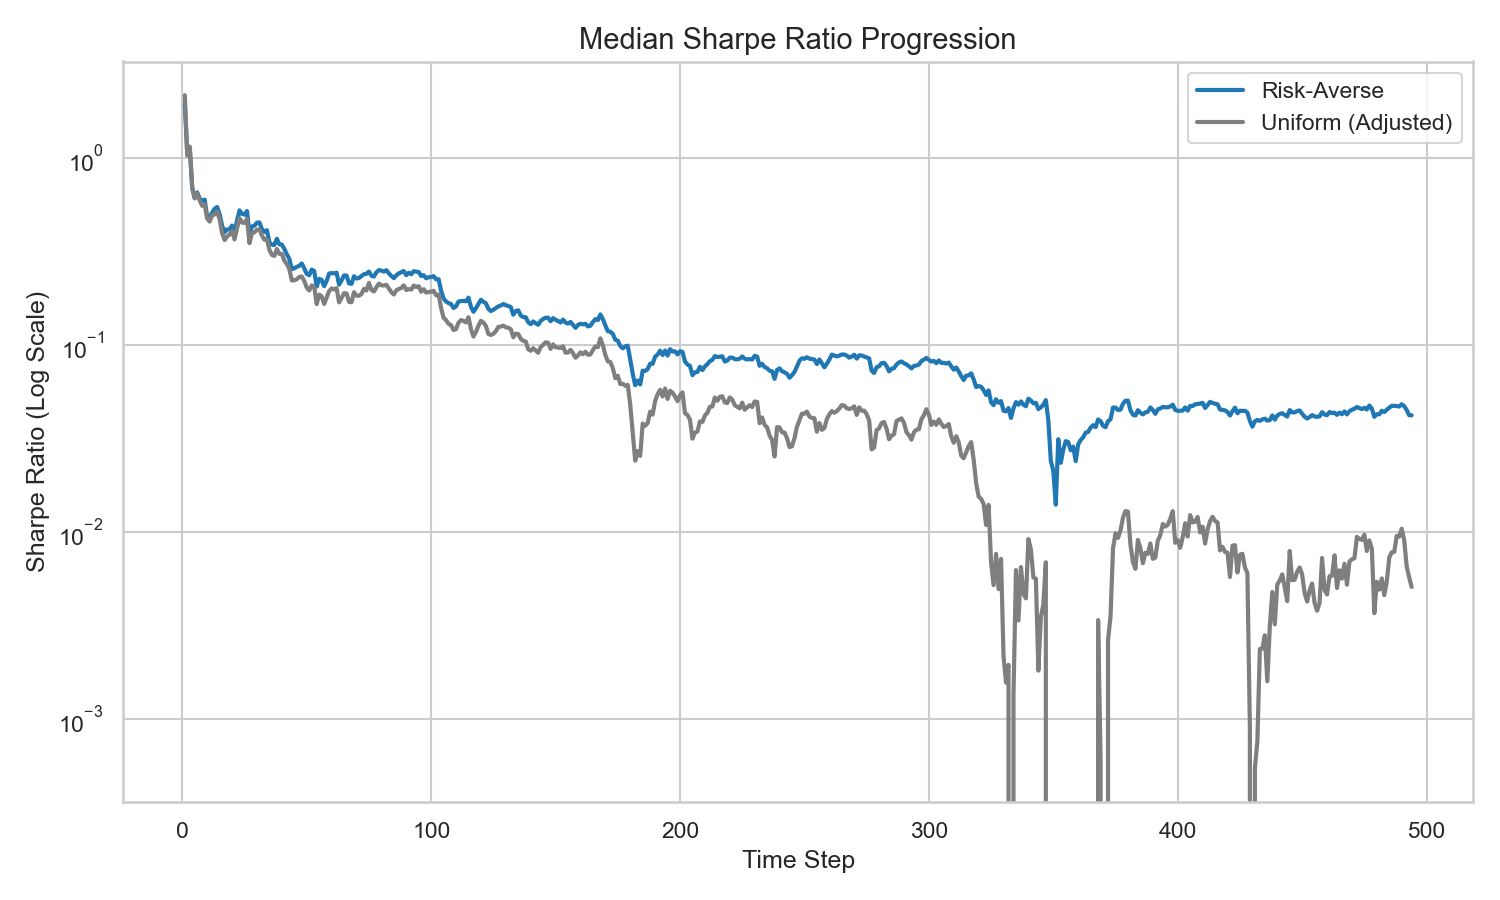
\includegraphics[width=\linewidth]{Images/median_sr_with_trc_u.png}
    \caption{Median Sharpe ratio progression for Risk Averse \& transaction costs included Uniform portfolios.}
    \label{fig:sr_plot_u}
    \end{minipage}
    \vfill

    \begin{minipage}{0.45\textwidth}
    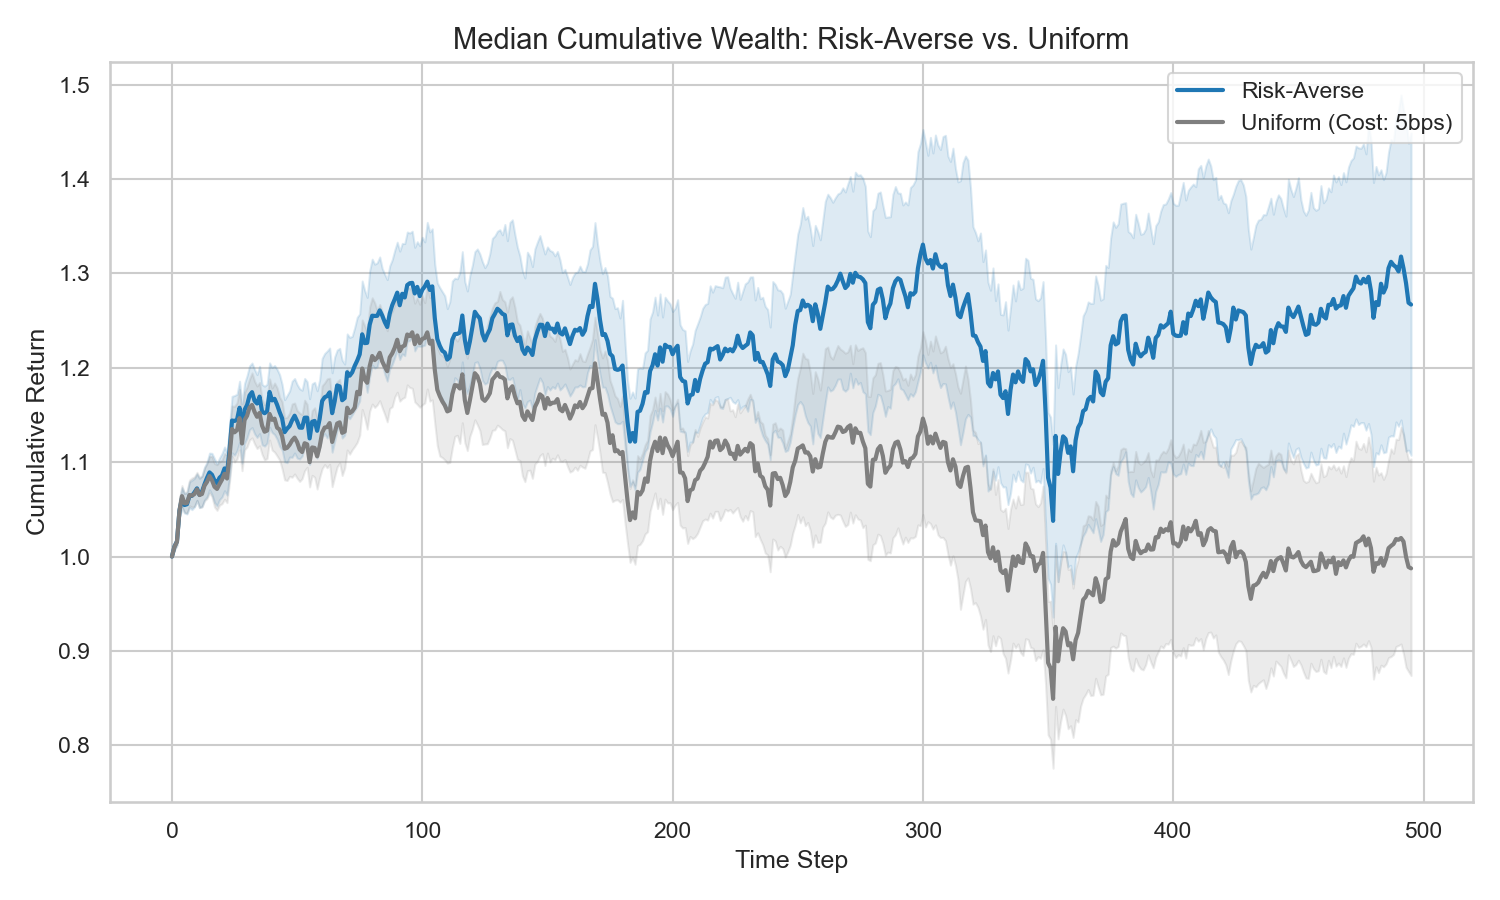
\includegraphics[width=\linewidth]{Images/cum_wealth_with_trc_u.png}
    \caption{Cumulative wealth for Risk Averse \& transaction costs included Uniform portfolios.}
    \label{fig:cum_wealth_u}
    \end{minipage}
\end{figure}

\begin{figure}[ht!]
    \begin{minipage}{0.45\textwidth}
    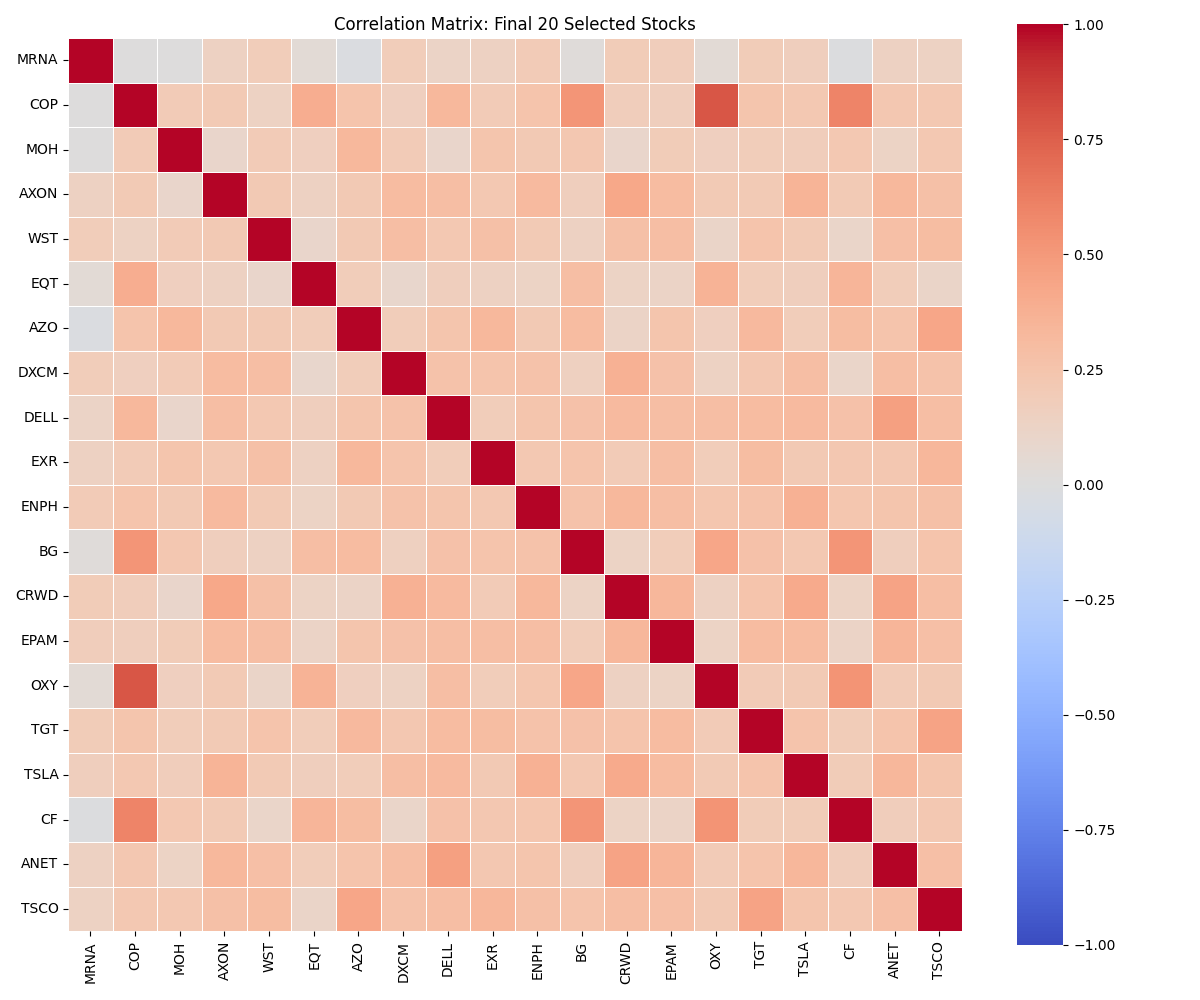
\includegraphics[width=\linewidth]{Images/selected_corr_matrix.png}
    \caption{Correlation matrix of the 20 selected stocks for our experiments.}
    \label{fig:corr_matrix}
    \end{minipage}
\end{figure}

\bl{We have performed a live test from March 1st 2026 to April 15th 2026 with a portfolio utilizing a mix of well established and more growth oriented companies with high market capitalization. Fig. \ref{fig:cum_wealth_live} shows the cumulative return in comparison to an additional benchmark S\&P500, the top 500 companies in the United States by market capitalization, during the trading period. Fig. \ref{fig:allocation_live} highlights the allocation into the selected stocks.}

\begin{figure}[ht!]
    \begin{minipage}{0.45\textwidth}
    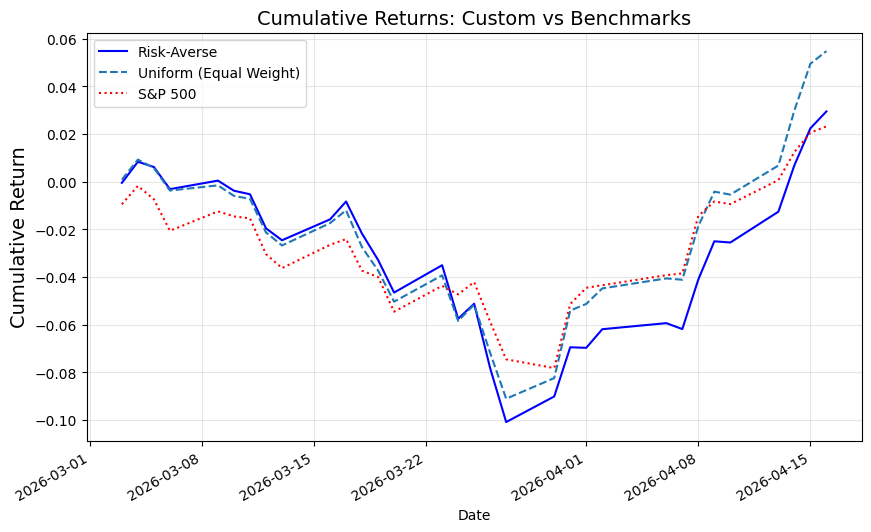
\includegraphics[width=\linewidth]{Images/live_returns.png}
    \caption{Returns comparison in live test. Risk Averse vs. Ideal Uniform portfolio vs. S\&P500 index benchmark.}
    \label{fig:cum_wealth_live}
    \end{minipage}
    \vfill

    \begin{minipage}{0.45\textwidth}
    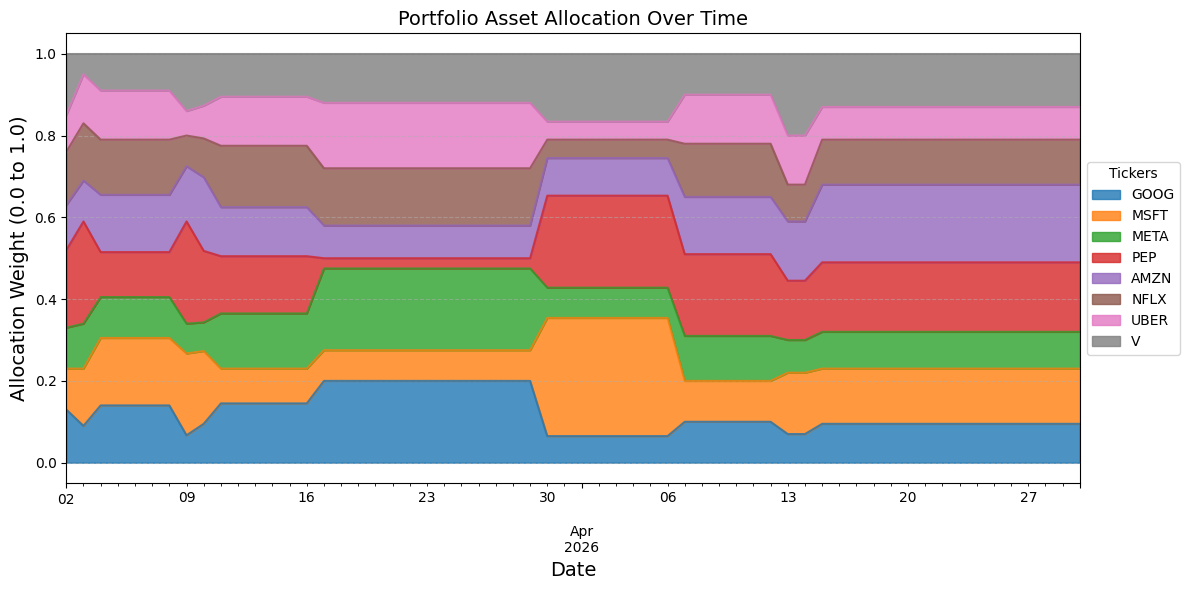
\includegraphics[width=\linewidth]{Images/live_allocation.png}
    \caption{Allocations of Risk Averse policy in live test.}
    \label{fig:allocation_live}
    \end{minipage}
\end{figure}

\bl{The relevant metrics are presented in Tab. \ref{tab:live_metrics}.}

  \begin{table}[ht!]
   \begin{minipage}{0.48\textwidth}
   % \centering
        \begin{tabular}{||l|r r r||} % Example table
        \hline
        & RA & U & S\&P500\\
        \hline
        max draw-down & -\textbf{0.108}& -0.099 & -0.077\\
        total return & \textbf{1.023} & 1.056 & 1.022\\
        SR & 0.074 & 0.133 & 0.069\\
        \hline
        \end{tabular}
      \caption{Comparison of live trading metrics.}
        \label{tab:live_metrics}
  \end{minipage}
\end{table}